% Options for packages loaded elsewhere
\PassOptionsToPackage{unicode}{hyperref}
\PassOptionsToPackage{hyphens}{url}
%
\documentclass[
]{article}
\usepackage{amsmath,amssymb}
\usepackage{iftex}
\ifPDFTeX
  \usepackage[T1]{fontenc}
  \usepackage[utf8]{inputenc}
  \usepackage{textcomp} % provide euro and other symbols
\else % if luatex or xetex
  \usepackage{unicode-math} % this also loads fontspec
  \defaultfontfeatures{Scale=MatchLowercase}
  \defaultfontfeatures[\rmfamily]{Ligatures=TeX,Scale=1}
\fi
\usepackage{lmodern}
\ifPDFTeX\else
  % xetex/luatex font selection
\fi
% Use upquote if available, for straight quotes in verbatim environments
\IfFileExists{upquote.sty}{\usepackage{upquote}}{}
\IfFileExists{microtype.sty}{% use microtype if available
  \usepackage[]{microtype}
  \UseMicrotypeSet[protrusion]{basicmath} % disable protrusion for tt fonts
}{}
\makeatletter
\@ifundefined{KOMAClassName}{% if non-KOMA class
  \IfFileExists{parskip.sty}{%
    \usepackage{parskip}
  }{% else
    \setlength{\parindent}{0pt}
    \setlength{\parskip}{6pt plus 2pt minus 1pt}}
}{% if KOMA class
  \KOMAoptions{parskip=half}}
\makeatother
\usepackage{xcolor}
\usepackage{graphicx}
\usepackage{subcaption}
\setlength{\emergencystretch}{3em} % prevent overfull lines
\providecommand{\tightlist}{%
  \setlength{\itemsep}{0pt}\setlength{\parskip}{0pt}}
\setcounter{secnumdepth}{-\maxdimen} % remove section numbering
\ifLuaTeX
  \usepackage{selnolig}  % disable illegal ligatures
\fi
\IfFileExists{bookmark.sty}{\usepackage{bookmark}}{\usepackage{hyperref}}
\IfFileExists{xurl.sty}{\usepackage{xurl}}{} % add URL line breaks if available
\urlstyle{same}
\hypersetup{
  pdftitle={Componenti connesse e Minimium Spanning Tree di un grafo},
  pdfauthor={Leonardo Toccafondi},
  hidelinks,
  pdfcreator={LaTeX via pandoc}}

\title{Componenti connesse e Minimium Spanning Tree di un grafo}
\author{Leonardo Toccafondi}
\date{February, 2023}

\begin{document}
\maketitle

\hypertarget{introduzione}{%
\section{Introduzione}\label{introduzione}}

Il grafo è una struttura che ha numerose applicazioni sia nei campi
dell'informatica sia in quelli dell'ottimizzazione.\\
Alcuni tipi di operazioni possibili su di essi sono le visite e la
ricerca di cammini, o insiemi particolari d cammini\\
Gli esperimenti che saranno eseguiti serviranno a esaminare due tipi
particolari di ricerche in un grafo: la ricerca delle componenti
connesse e la ricerca dell'MST (minimum spanning tree in inglese),
quest'ultima sarà effettuata attraverso l'uso dell'algoritmo di
Kruskal.\\
Ciò che ci interesserà scoprire maggiormente è il comportamento degli
algoritmi per queste ricerche all'aumentare dei nodi del grafo e della
probabilità di connessione tra gli stessi.\\
É necessario infatti che essi siano efficienti su grafi relativamente
estesi date le applicazioni reali, un esempio per le componenti connesse
è nell'analisi di immagini e quindi OCR, mentre la ricerca di un albero
di connessione minimo è un classico problema che si presenta nelle
telecomunicazioni.

\hypertarget{teoria}{%
\section{Teoria}\label{teoria}}

\hypertarget{grafi}{%
\subsection{Grafi}\label{grafi}}

Un grafo \(G\) è un insieme di elementi detti \textbf{vertici} (o nodi)
che possono essere collegati fra di loro tramite linee chiamate
\textbf{archi}. In particolare, si dice grafo la coppia ordinata di
insiemi \(G = (V, E)\), dove \(V\) è l'insieme dei vertici di \(G\) e
\(E\) è l'insieme degli archi di \(G\). Un grafo si dice
\textbf{orientato} (o \textbf{diretto}) se \(E\) è un insieme di archi
\emph{orientati}, cioè con una direzione (da sorgente a destinazione).
Viceversa, un grafo si dice \textbf{non orientato} (o
\textbf{indiretto}) se gli archi non sono orientati, dunque se la
connessione tra due vertici ij ha lo stesso significato della
connessione ji. Si definisce come grado di un vertice: numero di archi
che incidono nel vertice. Inoltre, ad ogni arco di un grafo può essere
assegnato un peso (che di solito corrisponde ad un numero reale, ma può
essere anche ristretto agli interi).

I grafi sono utilizzati come strutture dati al fine di rappresentare
relazioni tra elementi generici, espresse nel modo più semplice tramite
gli archi, che evidenziano le connessioni tra gli elementi.

\hypertarget{rappresentazione}{%
\paragraph{Rappresentazione}\label{rappresentazione}}

Un grafo può essere rappresentato con due tipologie di strutture dati:

\begin{itemize}
\item
  \textbf{Lista di adiacenza:} composta da un vettore \(Adj\) composto
  da \(|V|\) liste, una per ogni nodo, dove \(Adj[u]\) contiene tutti i
  vertici \(v\) t.c. \((u, v) \in E)\).

  La lista di adiacenza occupa uno spazio di memoria \(\Theta(V + E)\),
  e un tempo \(\Theta(u.degree)\) per determinare se due vertici
  qualsiasi \((u, v) \in E\). In questo caso \(u.degree\) rappresenta il
  \textbf{grado} del vertice (u).
\item
  \textbf{Matrice di adiacenza:} si introduce una matrice \(A\) di
  dimensione \(|V|\times|V|\), dove ogni elemento \((i,j)\) ha valore 1
  se \((i, j) \in E)\), cioè se il vertice \(j\) è adiacente a \(i\), e
  valore 0 altrimenti. La matrice di adiacenza occupa uno spazio di
  memoria \(\Theta(V^2)\), quindi peggiore rispetto alla lista, però
  consente di determinare se due vertici qualsiasi \((u, v) \in E\) in
  un tempo \(\Theta(1)\), in quanto è sufficiente accedere all'elemento
  \(A[u][v]\) e controllarne il valore. In generale, una matrice di
  adiacenza è più indicata per descrivere grafi \emph{densi} e con molti
  archi.
\end{itemize}

Per gli esperimenti svolti sono state utilizzate
\textbf{\emph{entrambe}} le strutture dati.

Per estrapolare ulteriori informazioni, si utilizzano le cosiddette
componenti connesse e l'albero ricoprente minimo (o Minimum Spanning
Tree in inglese), quest'ultimo tramite alcuni algoritmi, tra cui quello
di Kruskal. Tuttavia, è necessario prima introdurre una struttura dati
per degli insiemi disgiunti, nota anche come \emph{Union-find.}

\hypertarget{union-find}{%
\paragraph{Union find}\label{union-find}}

Gestisce una collezione di insiemi dinamici (disgiunti), ciascuno
identificato da un rappresentante, ovvero un elemento dell'insieme
qualsiasi, a patto che rimanga sempre lo stesso. Su questa struttura
dati possiamo operare con tre funzioni:

\begin{itemize}
\item
  MakeSet(x): aggiunge alla collezione un nuovo insieme creato a partire
  dall'elemento x;
\item
  FindSet(x): restituisce il rappresentante dell'insieme che contiene x;
\item
  Union(x,y): se
  \(x \in S_x, y \in S_y, \ \Rightarrow S \leftarrow S_x -S_y \bigcup \{S_x \cup S_y)\)
  Quindi aggiunge alla collezione un nuovo insieme contenente gli
  elementi degli insiemi di x e y, e poi elimina gli insiemi d'origine.
  Il rappresentante diventa uno degli elementi di \(S_x\) o di \(S_y\).
\end{itemize}

Dal punto di vista implementativo, la union-find viene realizzata
tramite \emph{liste concatenate}, dove ogni nodo ha come attributi
l'elemento dell'insieme, un puntatore al rappresentante ed uno
all'elemento successivo. Ogni lista contiene un puntatore alla propria
testa ed uno alla propria coda.

Per quanto riguarda invece la complessità temporale, possiamo facilmente
costruire una sequenza di m operazioni su n oggetti che richiede un
tempo pari a \(\Theta(n^2)\). Se il numero di elementi (e quindi il
numero di make\_set) è pari a \(n\) e \(m\) è il numero totale di
operazioni (\(m \geq n\) perché al massimo abbiamo \(n\) make\_set),
allora il costo di \(n\) make set è \(\Theta(n)\) e considerato che dopo
n-1 union abbiamo un solo insieme, allora il costo finale è
\(\Theta(n^2)\). Non solo, anche accodare una lista lunga ad una più
corta aumenta il tempo di esecuzione, in quanto sarà necessario
aggiornare \emph{ogni} rappresentante della lista che andiamo ad
accodare. Per questo si aggiunge un attributo size, al fine di
determinare quale delle due liste sia la più corta, e concatenare
quest'ultima alla lista più lunga. Con questa \textbf{\emph{euristica
dell'unione pesata}} una singola Union richiede tempo \(\Omega(n)\),
perché entrambi gli insiemi hanno \(\frac{n}{2}\) elementi.

\begin{quote}
\textbf{Teorema}: Il tempo con l'euristica per l'unione pesata per una
sequenza di \(m\) operazioni su \(n\) elementi è pari a \(O(m+n\lg n)\)
\end{quote}

In questo esperimento l'euristica dell'unione pesata è stata
implementata aggiungendo l'attributo size alla lista concatenata.

\hypertarget{componenti-connesse}{%
\subsection{Componenti connesse}\label{componenti-connesse}}

Dato un grafo \(G=(V,E)\), una componente connessa é un insieme
massimale di vertici \(C \subseteq V\) tale che per ogni coppia di nodi esiste un
cammino che li collega. Le componenti connesse \emph{partizionano} i
vertici in classi di equivalenza secondo la relazione \emph{``è
raggiungibile da''}. Un grafo è connesso se ogni coppia di vertici è
collegata attraverso un cammino. Sono utilizzate ad esempio per trovare
``oggetti'' all'interno di immagini, interpretando come nodi i singoli
pixel dell'immagine stessa L'algoritmo utilizzato all'interno di questo
esperimento si basa sull'utilizzo di union-find come struttura dati.

\hypertarget{albero-ricoprente-minimo-mst}{%
\subsection{Albero ricoprente minimo
(MST)}\label{albero-ricoprente-minimo-mst}}

Si tratti di un albero di connessione T (sottoinsieme dell'insieme di
archi \(E\) come un grafo non diretto \(G=(V,E)\)) in cui la somma dei
pesi dei suoi archi:

\begin{quote}
	\centering
\displaystyle  \(w(T) = \sum_{(u,v) \in T} \ w(u, v)\)
\end{quote}

sia minimo e connetta tutti i vertici. Un MST ha \(|V|-1\) archi, non ha
cicli e \emph{può non essere unico}.

Esiste un algoritmo generico che permette di costruire la soluzione e
consiste in creare un insieme vuoto di archi \(A\), per poi aggiungerne
progressivamente conservando l'invariante di ciclo:

\begin{quote}
''Se A é un sottoinsieme di qualche MST, l'arco \((u,v)\) é
\emph{sicuro} per A se e solo se \(A \cup (u,v)\) é sottoinsieme di un
qualche MST.''
\end{quote}

Da questo è possibile ricavare che al fine di ottenere un albero
ricoprente minimo sia necessario aggiungere solamente \(N-1\) archi
\emph{sicuri}, con \(N\) pari al numero di nodi.

Per ottenere l'algoritmo di Kruskal, che sarà utilizzato per gli
esperimenti, è necessario introdurre il seguente \emph{teorema}:

\begin{quote}
``Sia A un sottoinsieme di qualche MST, \((S,V-S)\) un taglio che
rispetta \(A\) e \((u,v)\) un arco leggero che attraversa \((S,V-S)\).
Allora \((u,v)\) é sicuro per \(A\).''
\end{quote}

Anche in questo caso per l'implementazione pratica viene utilizzata la
struttura dati \emph{Union-find.}

\hypertarget{implementazione-pratica}{%
\section{Implementazione pratica}\label{implementazione-pratica}}

Il programma è suddiviso in più file:

\begin{itemize}
\item
  graph.py si occupa della definizione dell'oggetto Node, che al suo
  interno contiene tutti gli attributi necessari, sia l'oggetto Graph,
  che corrisponde al nostro grafo. Il grafo viene popolato assegnando
  casualmente (in base ad un valore di probabilità) archi ad ogni nodo,
  portando ad uno il valore corrispondente nella matrice aggiogata. La
  matrice può anche essere equivalente alla matrice pesata, nel caso in
  cui la variabile booleana w sia posta a True al momento della
  creazione del grafo. Dopodiché viene inserito un vettore composto da
  {[}nodo u, nodo v, peso{]} (il peso nel caso di \emph{default} è posto
  ad 1). All'interno di questo file è presente anche la funzione
  sort\_edges, utilizzata nell'algoritmo di Kruskal per ordinare in base
  al peso gli archi.
\item
  linked\_list.py: in questo file vi è implementata la lista collegata
  utilizzata come base per la struttura dati union-find
\item
  union\_find.py: in questo file sono stati implementati gli oggetti e
  le funzioni necessarie al fine di rappresentare insiemi disgiunti
  dinamici.
\item
  cc.py: implementazione dell'algoritmo delle componenti connesse
\item
  mst.py: contiene l'implementazione dell'algoritmo di Kruskal
\end{itemize}

\hypertarget{esperimenti}{%
\section{Esperimenti}\label{esperimenti}}

In base a delle liste di dimensioni (espresse in percentuale), si vanno
a creare grafi di dimensione esponenziale \(2^n\), partendo da 0 fino ad
arrivare a 12 (quindi 2048 nodi). In un array sono state salvate le
probabilità di presenza di un arco tra i nodi (in particolare verranno
testate le probabilità 20\%, 40\%, 60\%, 80\%, 100\%).\\
I grafi presi in considerazione saranno grafi pesati generati
casualmente.\\
La dimensione dei grafi generati sarà sempre crescente ed inoltre
saranno testati vari modi di collegare i loro nodi. Per ogni dimensione
del grafo saranno generati diversi grafi, uno per ogni probabilità. La
crescita del numero di nodi sarà esponenziale, ad ogni ciclo sarà
raddoppiata fino ad arrivare ad un massimo di (2\^{}\{11\}). Per ogni
grafo generato prima di tutto verranno ricercate le componenti connesse
e sarà registrato il loro numero e il tempo di esecuzione. Dopodichè se
è stata trovata esattamente una componente connessa è possibile eseguire
la ricerca dell'MST con l'algoritmo di Kruskal. Per questo sarà
registrato solo il tempo di esecuzione. La registrazione dei valori
viene effettuata tramite la librerie pickle, mentre i grafici che ne
risultano sono stati ottenuti con la libreria matplotlib.

\hypertarget{ambiente-di-test}{%
\paragraph{Ambiente di test}\label{ambiente-di-test}}

\

L'esperimento è stato svolto~su un computer con le seguenti caratteristiche:

\begin{itemize}
\item
  Sistema operativo: Linux Mint 21.1 con kernel 5.15
\item
  CPU: Inter Core i7-9750H
\item
  RAM: 16 GB
\item
  Interprete Python: conda 22.11.1 e python 3.10
\item
  IDE: Pycharm Community Edition 2022.3.2
\end{itemize}



\hypertarget{risultati-degli-esperimenti}{%
\section{Risultati degli
esperimenti}\label{risultati-degli-esperimenti}}

\hypertarget{componenti-connesse-1}{%
\subsection{Componenti connesse}\label{componenti-connesse-1}}
\begin{figure}[h!]
	\centering
	\begin{subfigure}[b]{0.4\linewidth}
		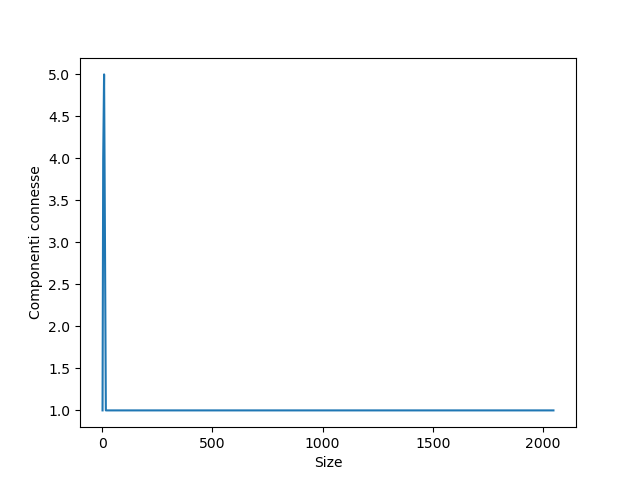
\includegraphics[width=\linewidth]{../img/cc/cc_number_p=20.png}
		\caption{Figura 1: p = 20}
	\end{subfigure}
	\begin{subfigure}[b]{0.4\linewidth}
		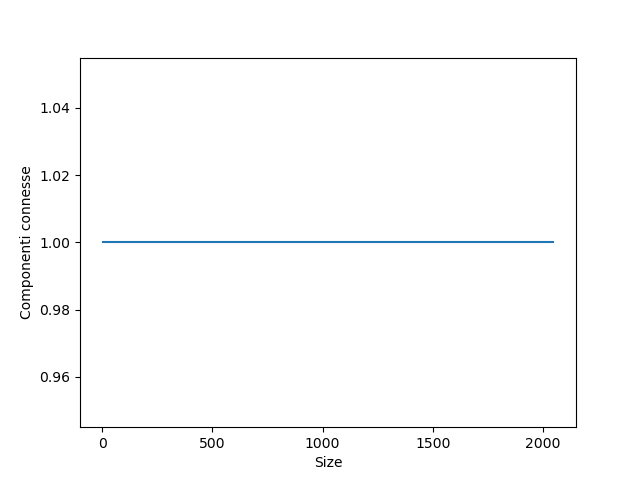
\includegraphics[width=\linewidth]{../img/cc/cc_number_p=80.png}
		\caption{Figura 2: p = 80}
	\end{subfigure}
	\caption{Componenti connesse trovate}
	\label{fig:CC_1}
\end{figure}

\begin{figure}[h!]
	\centering
	\begin{subfigure}[b]{0.4\linewidth}
		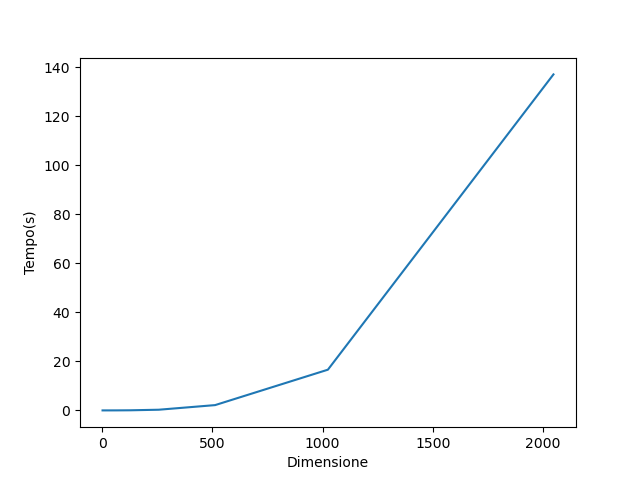
\includegraphics[width=\linewidth]{../img/cc/cc_time_p=20.png}
		\caption{Figura 3: p = 20}
	\end{subfigure}
	\begin{subfigure}[b]{0.4\linewidth}
		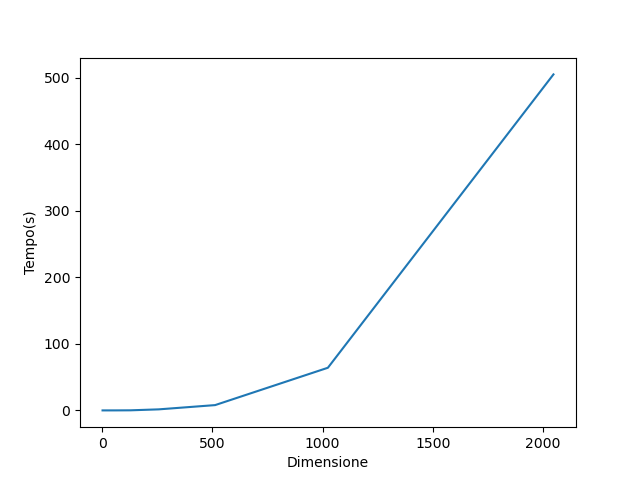
\includegraphics[width=\linewidth]{../img/cc/cc_time_p=80.png}
		\caption{Figura 4: p = 80}
	\end{subfigure}
	\caption{Tempo di esecuzione componenti connesse}
	\label{fig:CC_2}
\end{figure}

\newpage

\hypertarget{minimum-spanning-tree}{%
\subsection{Minimum spanning tree}\label{minimum-spanning-tree}}

\begin{figure}[h!]
	\centering
	\begin{subfigure}[b]{0.4\linewidth}
		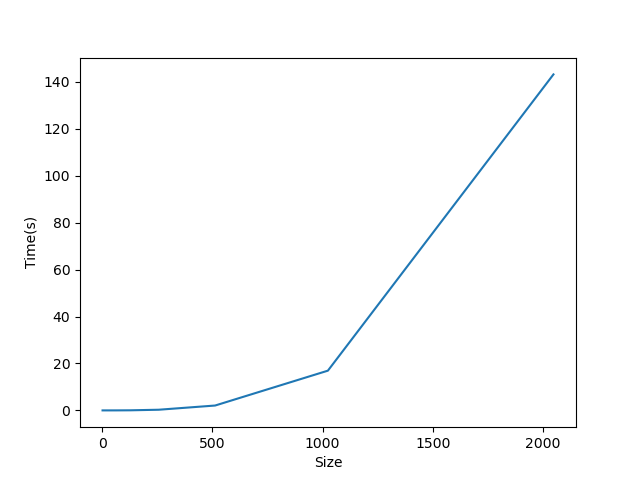
\includegraphics[width=\linewidth]{../img/mst/mst_time_p=20.png}
		\caption{Figura 1: p = 20}
	\end{subfigure}
	\begin{subfigure}[b]{0.4\linewidth}
		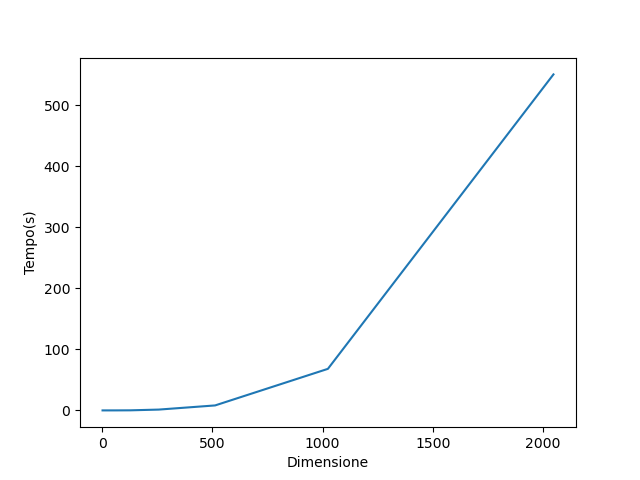
\includegraphics[width=\linewidth]{../img/mst/mst_time_p=80.png}
		\caption{Figura 2: p = 80}
	\end{subfigure}
	\caption{Tempo di esecuzione algoritmo di Kruskal}
	\label{fig:MST}
\end{figure}

\hypertarget{conclusioni}{%
\section{Conclusioni}\label{conclusioni}}

Esaminando i grafici nella figura 1 emerge che molto spesso nel
grafo generato si ha una sola componente connessa, soprattutto dal 40\%
di probabilità in poi.\\
Questo è particolarmente vero quando il numero di vertici del grafo è
superiore a 10-20, infatti anche se la probabilità di avere un
collegamento tra due nodi è abbastanza bassa in qualche modo sarà
generato un cammino che collega qualsiasi coppia di nodi, più o meno
lungo.\\
I tempi di esecuzione di questo algoritmo sono quelli attesi(come nelle
figure 2.1, 2.2) ovvero più che lineare rispetto al numero di archi,
cioè alla dimensione e alla probabilità di collegamento dei nodi.

Un comportamento molto simile lo ha anche il tempo di ricerca
dell'MST (figure 3.1, 3.2), anche se le sue costanti sono più alte.

\end{document}
